\documentclass[a4paper,11pt,titlepage]{article}
\usepackage{fullpage}
\PassOptionsToPackage{hyphens}{url}
\usepackage{graphicx}
%\usepackage[parfill]{parskip}

% define the title
\author{Adam Ku\v{c}era 4406028\\Maarten Duijn 1517279}
\title{Reverse Engineering and Detection Report}
\date{\today}
\begin{document}

% generates the title
\maketitle

\section{Initial understanding}
\subsection{Main features}
The essential part of the application is the Alitheia Core module itself, which provides the main functionalities and interfaces for plug-ins and other extensions. The most important features of the core are the following: initialization of the application and all related services, providing an interface for plugins, which can calculate project metrics, or import raw data, providing a web interface for administration and job submission, and lastly scheduling the metrics and other jobs parallel to each other.

%
%\begin{itemize}
%\item Initialization of the application and all related services.
%\item Providing an interface for plugins, which can calculate project metrics, or import raw data.
%\item Providing a web interface for administration and job submission.
%\item Scheduling the metrics and other jobs parallel to each other.
%\end{itemize}

\subsection{Important source code entities}
The product is split up into various services all individually manageable as an OSGi service. It thus stands to reason that the interface that all these services implement is one of the most import entities, and the class that manages the services is as well. These are AlitheiaCoreService respectively AlitheiaCore in the core package.

Another important entity is the eu.sqoos.service.db package, this package holds the database service interface as well as all the objects used by the object relational mapper.

The main purpose of Aliteia core is to enable software engineering research. It does this by letting plugins calculate metrics over projects based on data from several sources. As a consequence the interface for plugins: AlitheiaPlugin and the class implementing basic plugin functionality: AbstractMetric belong in the list of the most important entities.

\subsection{First impression}
The very first impression of the software we got was by inspecting the website which had some clear high level documentation but seemed to be very out of date. This documentation trend continues throughout the project, overall the software seems to be moderately well documented but there is definitely room for improvement. Some examples are: not being able to open the database schema without debugging the software, various commenting styles and missing method, package or class documentation. 

We did like the overall design of the software itself, it seems straightforward with a good level of abstraction and a clear separation of responsibilities. The testing for the software on the other and was very underwhelming, unit tests are very scarce, and even when they do exist are short, not documented and have no clear result message. The worst part about this is that the implementation reflects this fact, in general, code is not easily testable due to long and complex methods.

\subsection{Feasibility of reengineering}
We do think reengineering is feasible, the main reason for this is that the overall architecture looks quite good. The product is well designed, relatively easy to understand and for a research product easy to run. The design patterns used throughout the product are applied in an appropriate way which makes the product relatively maintainable, extensible and flexible.

\section{Exceptional entities}
\subsection{Inheritance structure}
The general inheritance structure is that when a class is used in some way by other classes it gets an interface that is placed in an abstract package with other interfaces for classes from the same package. When a class is not used by classes outside the package but only by classes inside the package, an interface is defined for this class in the packages itself.

Plugins and metrics used in calculation and data retrieval have to implement a special interface or extend a class already providing certain basic methods making the software easily extendible.

\subsection{Exceptional packages}
Package eu.sqooss.service.db is the biggest package in the application, as it contains the highest number of classes. The whole package is responsible for maintaining the database connection and most of the classes represent Data Access Objects mapping different application entities to the database. These DAOs usually have a lot of getter and setter methods, which is diagnosed as a flaw by the tools, but we do not consider as a big problem, as DAOs usually look that way.

On the other hand, package eu.sqooss.plugins.updater.svn responsible for synchronizing metadata in database with Subversion repository contains only one very long class.

Package eu.sqooss.service.util contains basic utility functions e.g. manipulating with strings or files. However, this package does not follow the inheritance structure mentioned above and it already contains implemented functions. Similar case might be main eu.sqooss.core, which provides initialization and service loading functionalities and therefore does not implement any interface.

\subsection{Exceptional classes and methods}
We found several classes, which might be considered as God classes, which means, that these classes have too much responsibilities. Classic example of such a class is AlitheiaCore, which is responsible for loading and starting all of the application components. Other classes also resemble the God class anti-pattern. Class AbstractMetric is such a case, as it is responsible for a lot of common features connected to metrics, is widely used throughout the application and also uses a lot of methods from other classes.

Classes ProjectView or PluginsView are part of the presentation layer of the application and therefore contain rendering methods. However, these rendering methods are usually very long and sometimes mix the presentation data itself with business logic.

%There are more classes with pretty long and complex methods. For example UpdateServiceImpl contains very long and complex update() method, which is responsible for the whole updating process, when something changes in raw data sources. This method should at least be split into different methods, as it is performing different tasks in sequence.
%
%More very complex methods exist in the application. In class ContributionMetricImpl there is quite long run() method with deeply nested statements. Also Structural class contains serveral complex methods, which are e.g. using if statements inside switch statements, which has bad effect on the complexity.

SVNUpdaterImpl class might have a feature envy, as it uses a lot of methods from other objects. On the other hand FileUtils class is exactly the opposite, as it is used by a lot of other classes. That is however expected from an utility class.

\section{Details}
\subsection{Basic elements to compose a scene}
All basic HTML sources for a scene are in the src/main/resources folder. These files are calling rendering methods mostly from eu.sqooss.impl.service.webadmin package, but also from other packages, from which the information should be viewed. All of these HTML files include the same basic structural files such as header.inc, menu.inc or sidebar.inc. It means, that all these files contain the same head and tail, which might mean possible duplicate code and option for future refactoring.

\subsection{Rendering of scenes}
The application is leveraging Apache Velocity to render its web interface. AlitheiaCore class first starts the webadmin service, which initializes HTTP service and starts the Velocity, which loads all the template resources. Template resources then call respective rendering methods for the information it needs to display, e.g. RenderFailedJobs(). The interaction with the user is handled via GET and POST requests using AdminServlet class.
%
%\subsection{Collision detection}
%We are not exactly sure what is meant by a collision in this domain, so we suppose, that it is an event, when the raw project source is updated and therefore there is a conflict between this raw data and metadata in application database. An update of the database is handled by given Updater for the specific raw source. Such an update is started only manually from the interface, ProjectView’s render() method parses the request to update an project and this update is performed through UpdateProject class in the Admin service.

\section{Problem detection}

\subsection{Single Responsibility Principle violations}
The AbstractMetric class is a classic example of an SRP violation, the class provides implementations for the OSGi bundle information retrieval, logging services, database access methods and more. The problem could be said to lie in AlitheiaPlugin as well since the interface forces implementation in a single class to a certain degree. The best solution would be to split up the interface and thus class hierarchy and make each responsible for a single feature (ie. logging, database access, plugin management)

Many of the render and update methods in the product are very long indicating there might be problems with the SRP. We picked two of these: PluginsView render and UpdateServiceImpl update as examples of SRP violation. The render method is extraordinarily long with 867 lines of code, has a high complexity with a maximum nesting of 10 and places 415 outgoing method calls. The method is responsible for rendering different views from lists of plugins and rendering HTML for updating and configuration. By splitting up these different functions into a number of separate methods responsible for a single function most of the problems will be solved.

The same goes for the UpdaterServiceImpl update method, with 226 liines of code and a cyclometic complexity of 36. The method performs a topological sort which should most certainly be a standalone method. Such an algorithm is a very likely candidate for bugs and should be easily testable.

\subsection{Liskov Substitution Principle violation}
An example of an LSP violation is the class UpdaterJob, which is a descendant of Job class violates the LSP, more specifically its usage in the application. When the update job is started in update() method in UpdateServiceImpl class, it is always added as a dependency to another already scheduled update jobs. It iterates over all scheduled jobs and using instanceof operator, it asks only for instances of UpdaterJob class.

The idea of course makes sense, because other scheduled jobs of other types do not depend on these update jobs, however this is a violation of the LSP, because to follow this principle, all jobs should look to the same to the application and instanceof should not be necessary to use.

\subsection{Open Closed Principle violation}
We have been able to detect one small violation of the OCP. It concerns the class UpdaterServiceImpl, which extends the class AlitheiaCoreService. This parent class has an explicit requirement that all its descendants should implement an empty constructor (which is different from omitting the constructor implementation, which results into calling the constructor of super class). This might cause problems in the future, as this means, that UpdaterServiceImpl might not be used in place of all AlitheiaCoreService subtypes thus it violates the OCP.

\subsection{Dependency Inversion Principle violation}
DBServiceImpl class contains implementations for all different types of databases, which is a violation of DIP. In Java, the access to these databases is more or less the same thanks to JDBC driver, but exact implementation for each technology should be in different class and a super interface or an abstract class should be introduced. That would make it easier to add a new technology to the system without the need of editing (and testing) the whole complex DBServiceImpl class.

Being more abstract, the whole application might not be using only relational databases as the storage in the future, but also different storage type (for example file storage). Therefore another interface representing a DataAccess class could be added and the database service would be just implementation of this interface. Possible change of the storage technology in the future would be then very easy.

\subsection{Acyclic Dependency Principle violation}

\begin{figure}
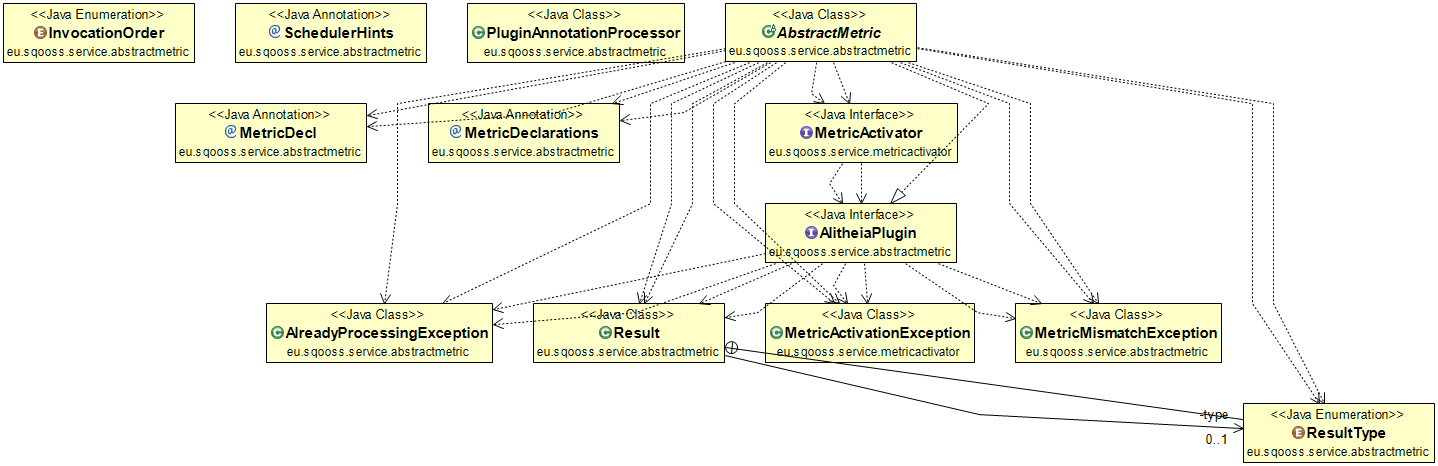
\includegraphics[scale=0.3]{class_cyclic_dependency}
\centering
\caption{Class diagram of AbstractMetric and MetricActivator packages}
\label{fig:classmetrics}
\end{figure}

\begin{figure}
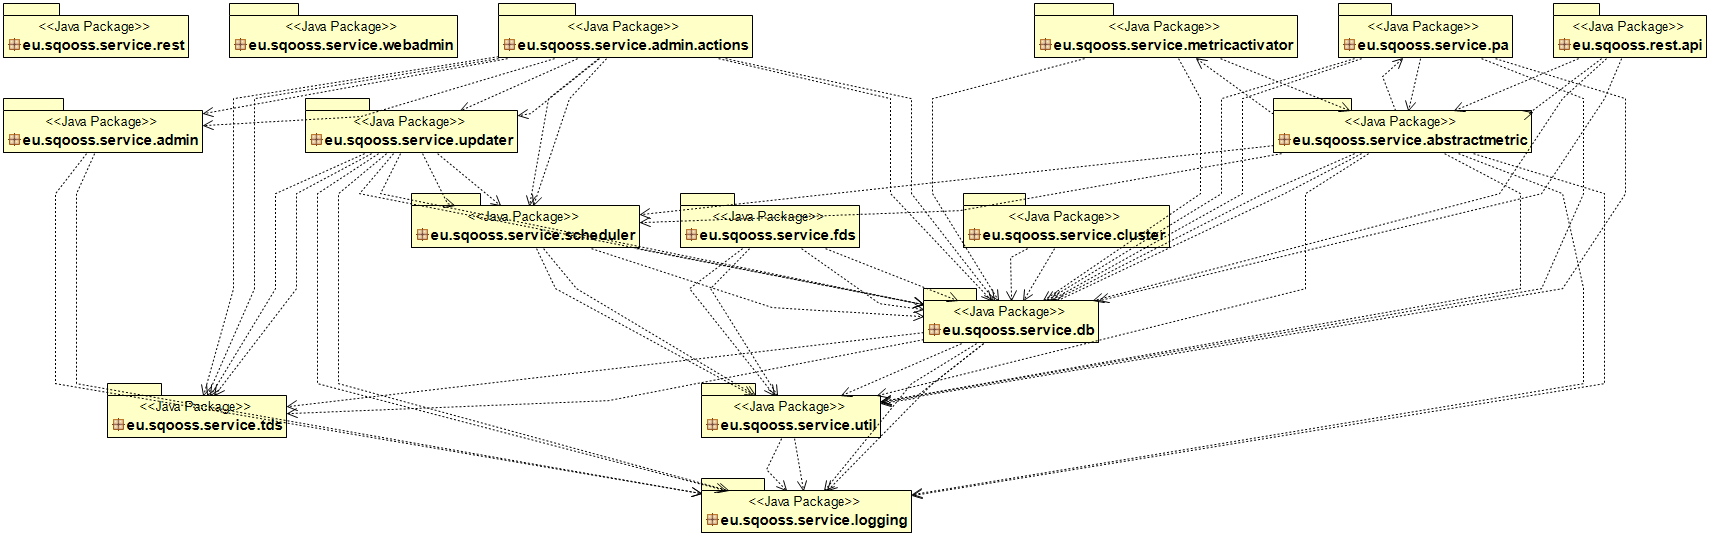
\includegraphics[scale=0.25]{package_diagram_core_no_impl_no_core}
\centering
\caption{Package diagram showing a subset of the packages in Alitheia Core}
\label{fig:package}
\end{figure}

A clear example of a violation of the Acyclic Dependency Principle is the relation between the AbstractMetric and MetricActivator packages. As shown in figure \ref{fig:classmetrics}, classes in both packages are used by each other and thus dependent on each other. There seem to be more problems regarding the AbstractMetric package as this package has another cyclic dependency with the pa package, shown in figure \ref{fig:package}. The AbstractMetric package depends on the pa package and vice versa.

\subsection{Duplicated Code}
The Don't Repeat Yourself principle is violated in a number of places throughout the product. The most clear example of this is the duplication in the DBServiceImpl class. In this class the doSQL method with approximately 30 lines is effectively copied into the callProcedure method.

A less severe type of duplication: sibling duplication is demonstrated by the SVNUpdaterImpl class, in this class the replayLog method is very similar to the GitUpdater replayLog method. The duplication is understandable, one might want to clearly separate functionality in the raw data handling classes. However by introducing a separate class higher in the class hierarchy for versioning systems with similar functionality (ie. Git, SVN, Bazaar) this duplication would not be necessary.



\end{document}